\documentclass[12pt]{article}
\usepackage[margin=1.0in]{geometry}
\usepackage{graphicx}
\usepackage[pdftex]{hyperref}
\usepackage{wrapfig}
\usepackage{float}
\usepackage{enumitem}
\usepackage{textcomp}
\usepackage[english]{babel}
\usepackage{csquotes}
\usepackage[document]{ragged2e}
\usepackage[utf8]{inputenc}
\usepackage{indentfirst}
\usepackage{nicefrac}
\usepackage[dvipsnames]{xcolor}

\emergencystretch=\maxdimen
\hyphenpenalty=10000
\hbadness=10000
\MakeOuterQuote{"}
\renewcommand{\baselinestretch}{1.2}
\setlength\parindent{0.5in}
\setlength\RaggedRightParindent{\parindent}
\setlength\parskip{1em}
\let\supscr=\textsuperscript
\newcommand{\graytext}[1]{{\leavevmode\color{gray}#1}}

\begin{document}
\begin{titlepage}
    \centering
    \vspace{15cm}
    {\huge\bfseries Subsystems Report \par}
    \vspace{1cm}
    {\scshape\Large Jonathan Sumner Evans\par}
    \vfill
    {\scshape\large Section U\par}
    {\large \today\par}
    \vfill
\end{titlepage}

\tableofcontents

\graytext{
    \pagebreak
    \section{Introduction}
    A food desert is an area where access to fruits and vegetables is limited, too expensive, or
    nonexistent due to a lack of grocery stores and farmers markets within a convenient walking
    distance \cite{cdc-food-deserts}. People living in food deserts often rely on fringe food
    retailers and discount stores, such as gas stations and dollar stores, for food. These retailers
    tend to sell high-fat and processed foods which contributes to higher rates of obesity and
    diabetes in those food desert areas. According to the US Department of Agriculture, there is a
    food desert in the Wheat Ridge area located between Wadsworth, 32\supscr{nd} Avenue, and
    38\supscr{th} Avenue \cite{usda-food-deserts}.

    The team’s goal is to empower English and Spanish speaking Wheat Ridge residents over 65 years
    in age who live in a food desert and rely on food stamps to utilize a self-sustaining plant
    growing system. Most of the system will come prepackaged for safe installation and use. It will
    also partially use materials that can be sourced in the Wheat Ridge neighborhood. The net cost
    will be neutral or better after two years of plant harvest and will include features that
    consider the potential physical limitations of the stakeholders.

    \section{Solution Description}
    The team’s design addresses the problem with a system composed of five distinct and
    interconnected subsystems. The structural subsystem is a three-tiered structure that is compact,
    lightweight, and cost-effective so that the stakeholder can easily install and maintain it. With
    it’s 12 hole design and the reservoir at it’s base, the structure is the key connection between
    the hydroponic soda bottle system and the watering system.

    The watering system consists of two symbiotic subsystems: the reservoir and the cascading water
    system. The reservoir system uses four separate water tanks each of which correspond a growing
    stage in the plant cycle. The water is delivered to each plant by pumping water to the bottles
    in the top tier of the structure; the water then cascades down to the next two rows through
    tubing that connects the bottles together. Water drains from the lowest bottle back into the
    reservoir. This system only requires the stakeholder to refill the reservoirs one time per week.

    The nutrient subsystem is housed partially within the reservoir. Along with the structure and
    watering system, the stakeholder will receive packages of pre-measured nutrients that correspond
    to the growing cycle of the plants. By using a color-coding system, the nutrient system will be
    easy to understand regardless of the stakeholder’s native language. The stakeholder simply has
    to fill the reservoirs with the nutrients and water which will then be delivered to the plants
    via the water delivery system.

    Finally, the hydroponic (soilless) soda bottle system is composed of re-purposed 2-liter soda
    bottles and materials that can easily be sourced in the Wheat Ridge food desert. We chose a
    hydroponics system because they use up to 90\% less water, so they can be watered less often and
    are typified by less insects, a more controlled environment, and a steady harvest
    \cite{j-camas}. The soda bottles are the foundation for the snow peas, lettuce, and spinach to
    grow. The water-nutrient mixture is pumped into the bottles and is carried to the plant via a
    wick. This design prevents the stakeholder from overwatering and underwatering the plants and
    lowers the cost of the entire system by using easily-sourced substrate instead of soil.  The
    final solution also includes a tool which will allow the stakeholders to easily construct the
    bottle systems themselves despite their physical limitations. These five interconnected
    subsystems comprise the team's final solution (shown in Figure 1): an elegant, easy-to-maintain 
    food growing system designed with the stakeholders’ needs in mind.

    \pagebreak
    \begin{figure}[H]
        \centering
        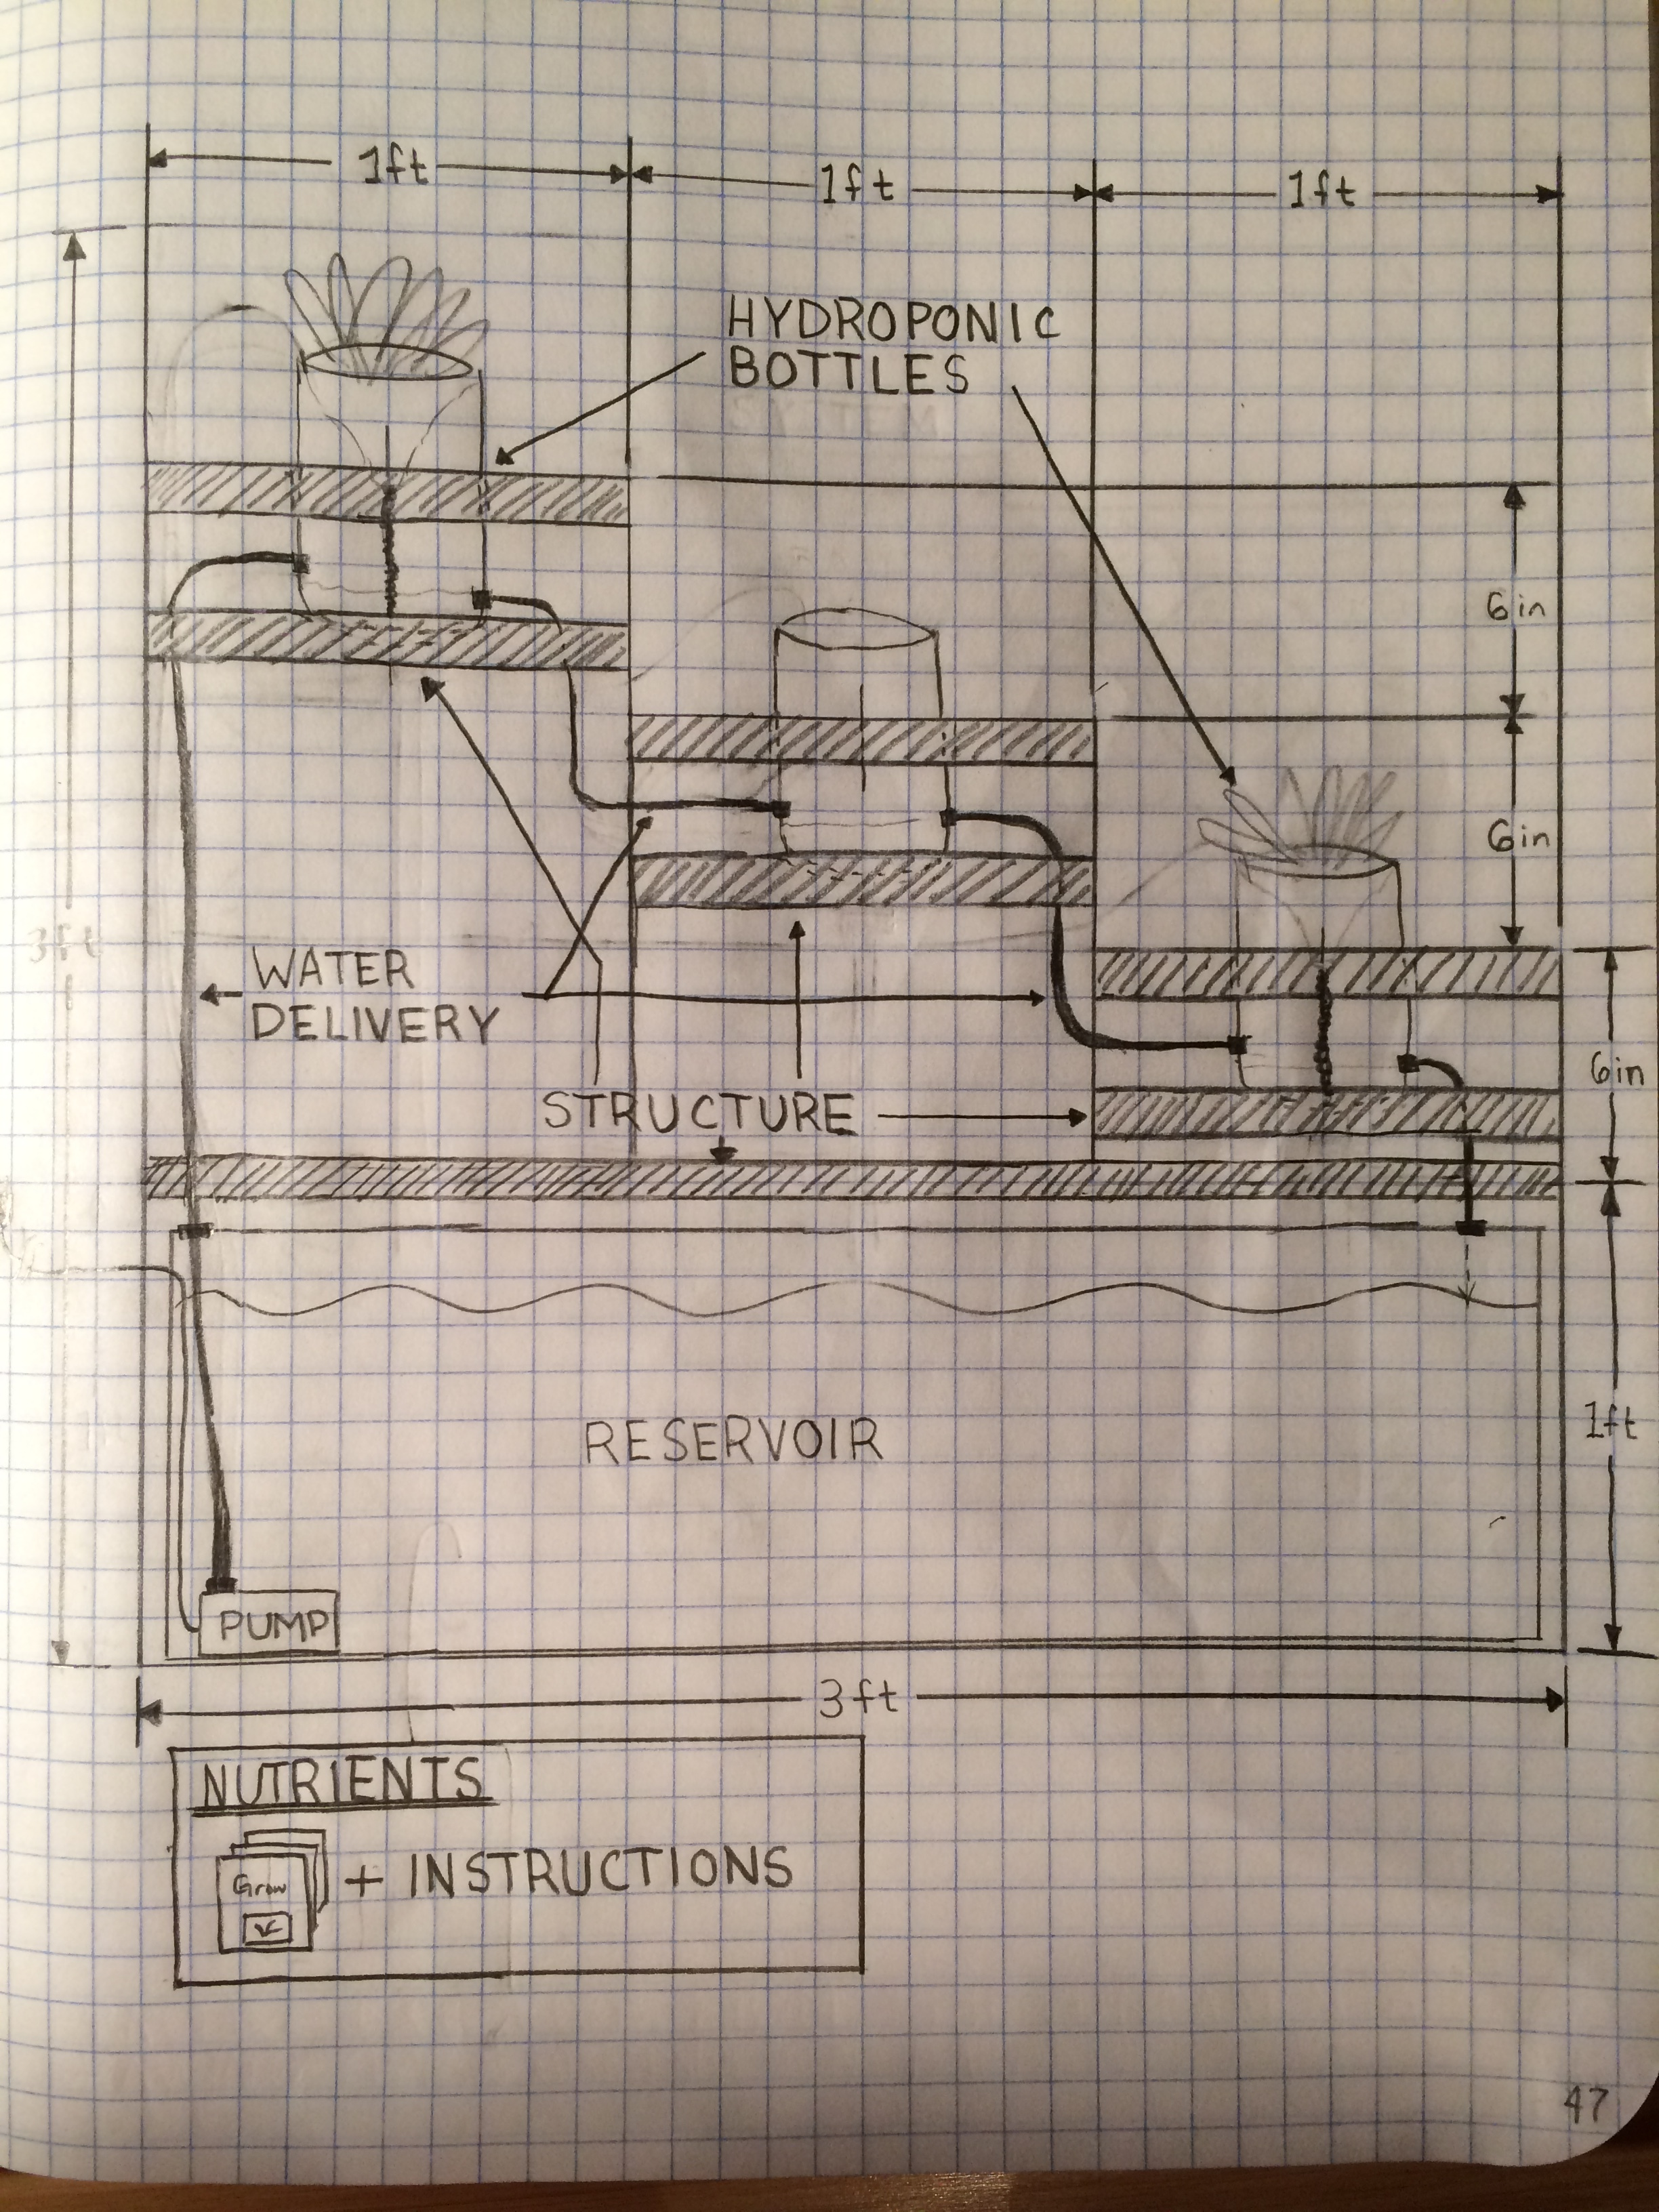
\includegraphics[width=163mm]{resources/system-overview.jpg}
        \caption{System Sketch Showing Each Subsystem}
    \end{figure}
}

% ===== TODO =====
% - Do a search for subsystem
% - Three citations (1 done)

\section{Subsystem Description}

% Describe your subsystem functionality and key components.

The water delivery subsystem is the sole mechanism for transporting nutrients and water from
the reservoir to the soda bottles. This subsystem is critical to the overall system because if water
and nutrients are not delivered to the bottles, the plants cannot grow and no food can be produced.
The water delivery subsystem is comprised of four separate water circulation systems, one for each
nutrient stage. This helps facilitate the system's modular design. Each circulation system
corresponds to a single column of bottles and distributes water to each bottle in the column (see
Figure 1).

Since we are using a wicking mechanism to transport water and nutrients from the bottom of the
bottle to the plant, the circulation system does not have to run continuously, it merely needs to
maintain the water level in each bottle. Because of this, the design requires the pumps to be on a
timer which allows the water to run for a few minutes every hour. This solution decreases the
environmental footprint of the system and also reduces operating costs for the stakeholder.
Additionally, if there is a power outage and the pumps stop operating for a period of time, the
system will remain stable unless the water in the individual bottles runs out.

Many of the water delivery system's components are interfaces with other subsystems. The only
component of the design specific to the water deliver system is the tubing. The tubing carries water
and nutrients from each of the four reservoirs to the uppermost bottle. The tubing also carries
water from one bottle to the next in each column until the water drains out of the lowest bottle in
the column and back into the reservoir through another tube. In the final design, $\nicefrac{1}{2}"$
tubing will be used. This diameter was chosen for two reasons:

\begin{enumerate}

    \item The pumps that the team is considering have $\nicefrac{1}{2}''$ fittings.

    \item There are many options for $\nicefrac{1}{2}''$ bulkheads on the market. From my online
        searches, $\nicefrac{1}{4}''$ bulkheads are less common. These bulkheads are the primary
        interface point between the water delivery system and the hydroponic bottles (see Subsystem
        Interfaces for details).

\end{enumerate}

% Physical properties, including dimensions, material type, specifications, weight, and
% construction.

The tubing in the final product will be black to reduce the water's exposure to light. Exposure to
light causes algae growth \cite{doe-washington} and since one of the system's requirements is that
algae growth is prevented, this precaution is necessary.

% Include sketches with dimensions instead of long physical descriptions.
As shown in Figure 2, there is a total of $3'$ of tubing between the pump and the uppermost bottle.
$7\ \nicefrac{3}{4}''$ of the tubing is inside the reservoir and $2'\ 4\ \nicefrac{1}{4}''$ is
outside the reservoir. Figure 3 shows that there is a total of $1\ \nicefrac{1}{2}'$ of tubing
between each bottle: $\nicefrac{1}{2}'$ horizontally and $1'$ vertically.

\begin{figure}[H]
    \centering
    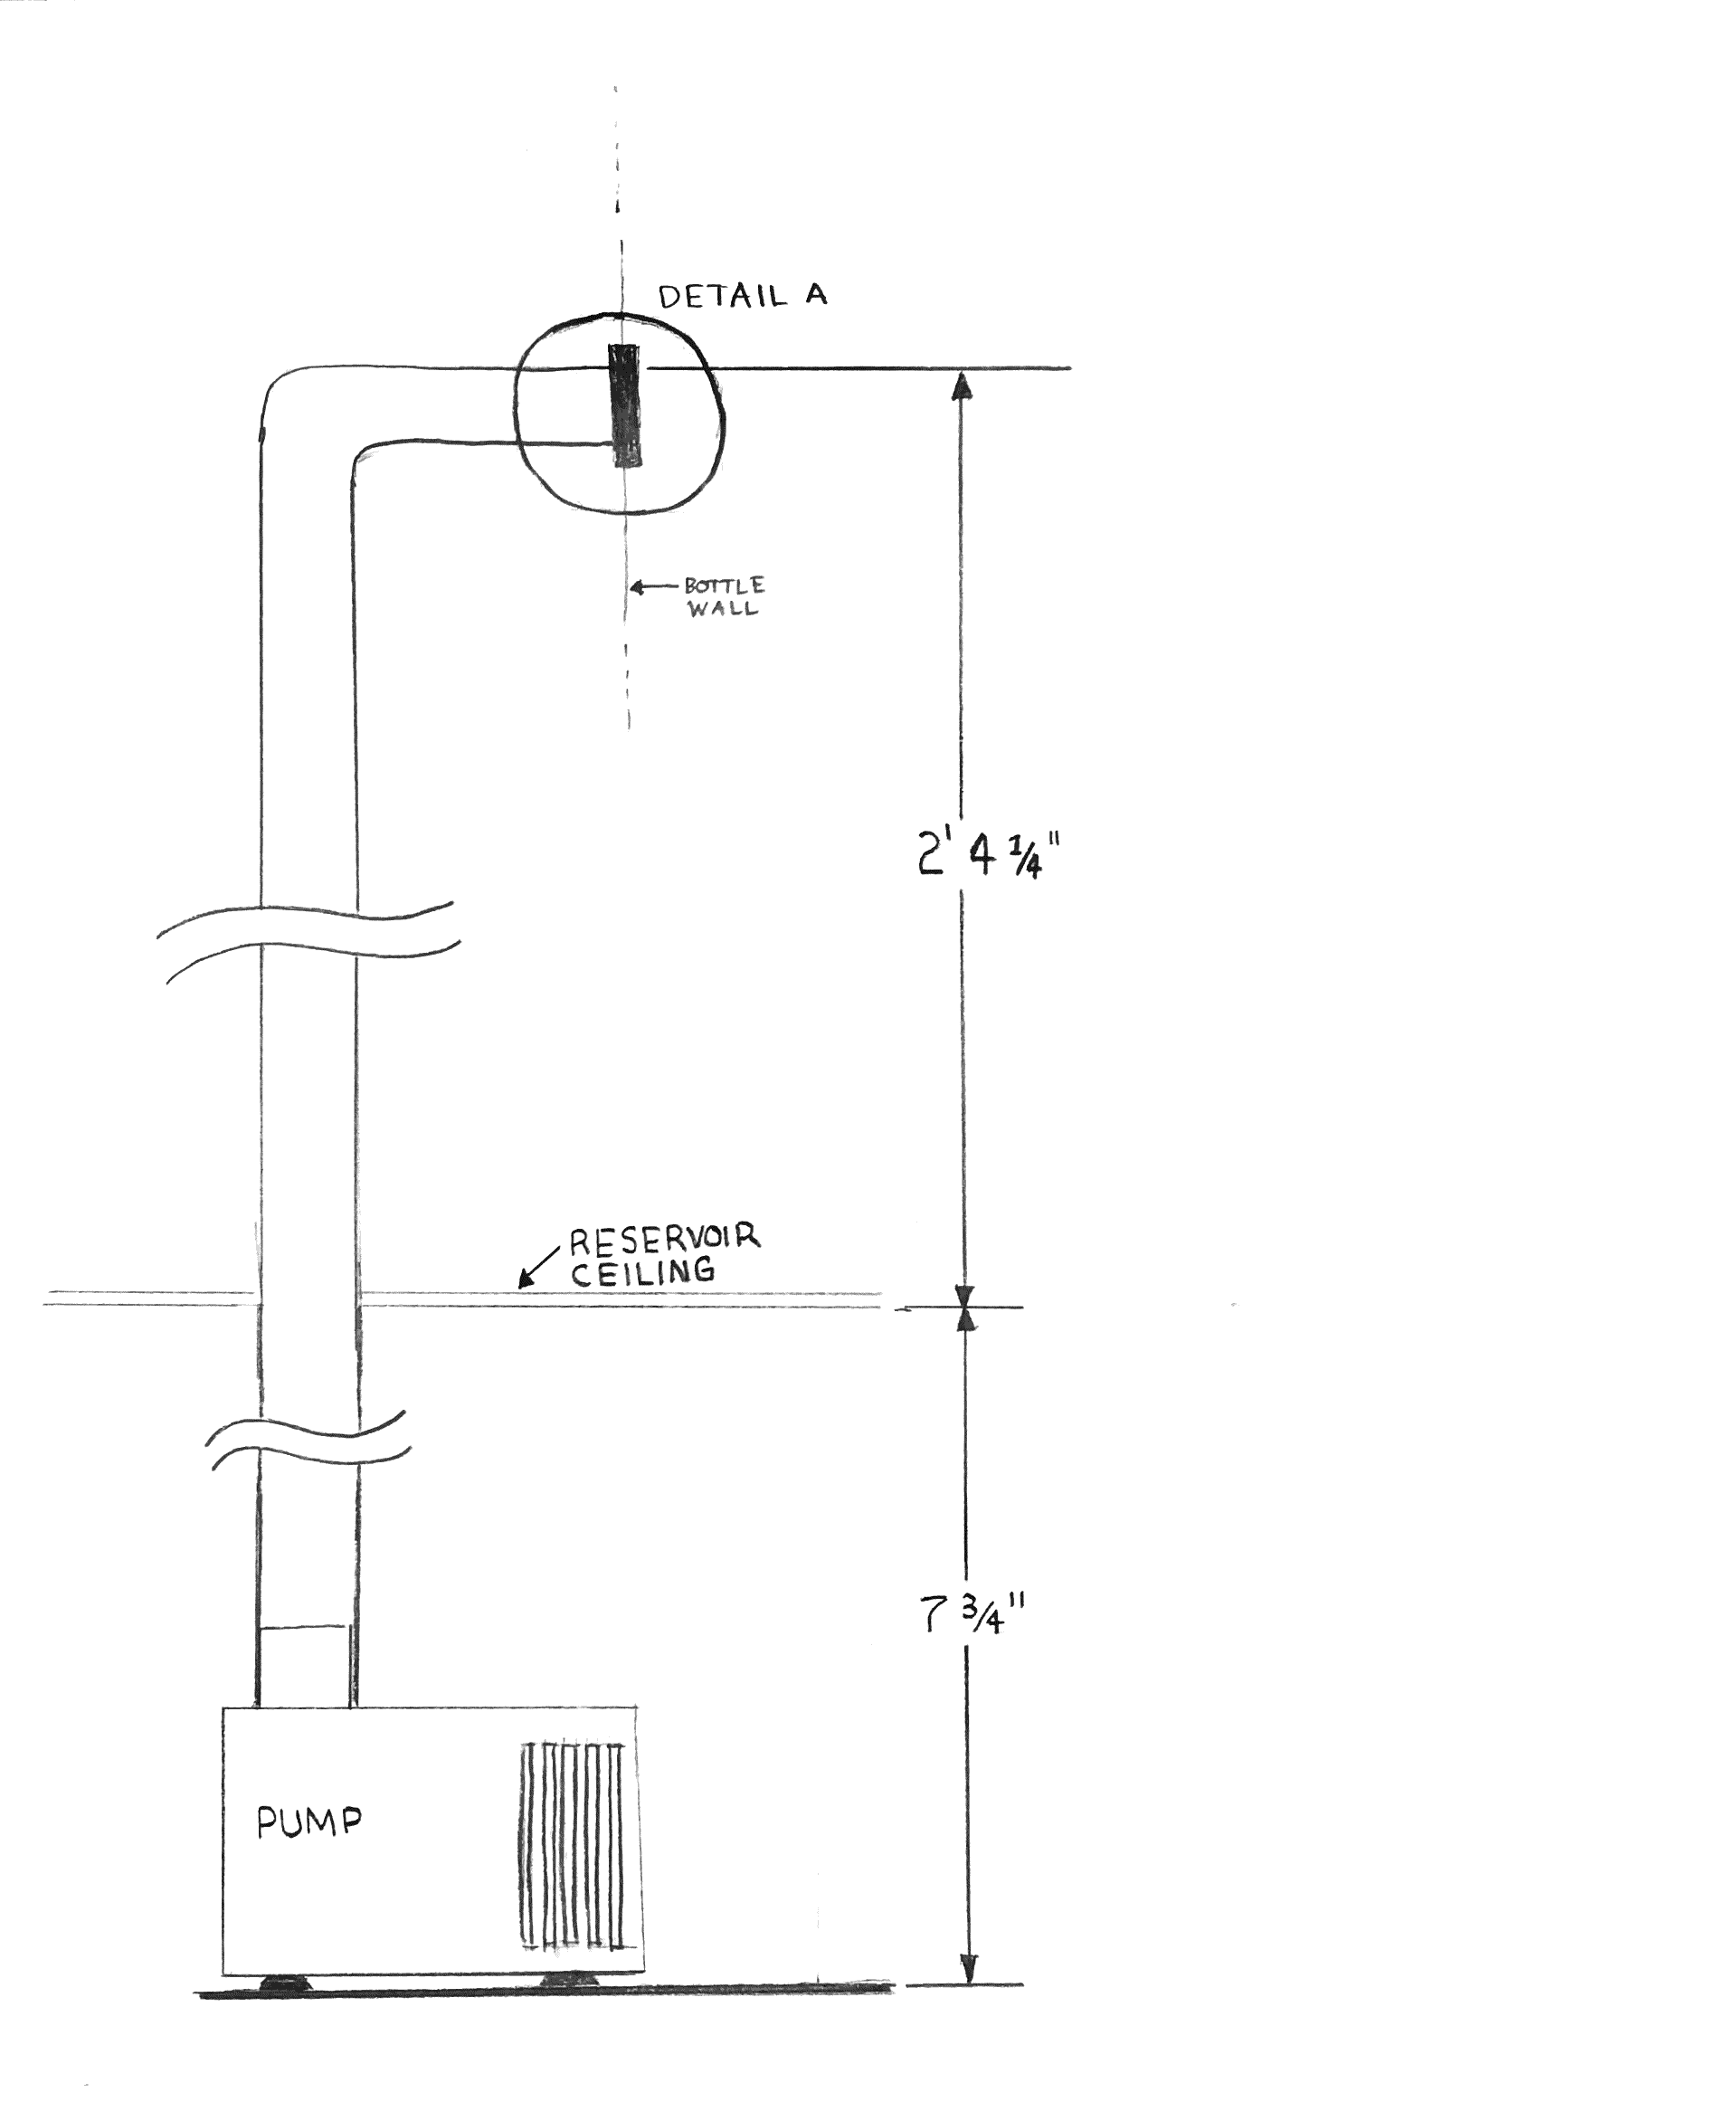
\includegraphics[width=145mm]{resources/tubing-pump-to-bottle.png}
    \caption{Dimensions of Tubing from Pump to Bottle}
\end{figure}

\pagebreak
\begin{figure}[H]
    \centering
    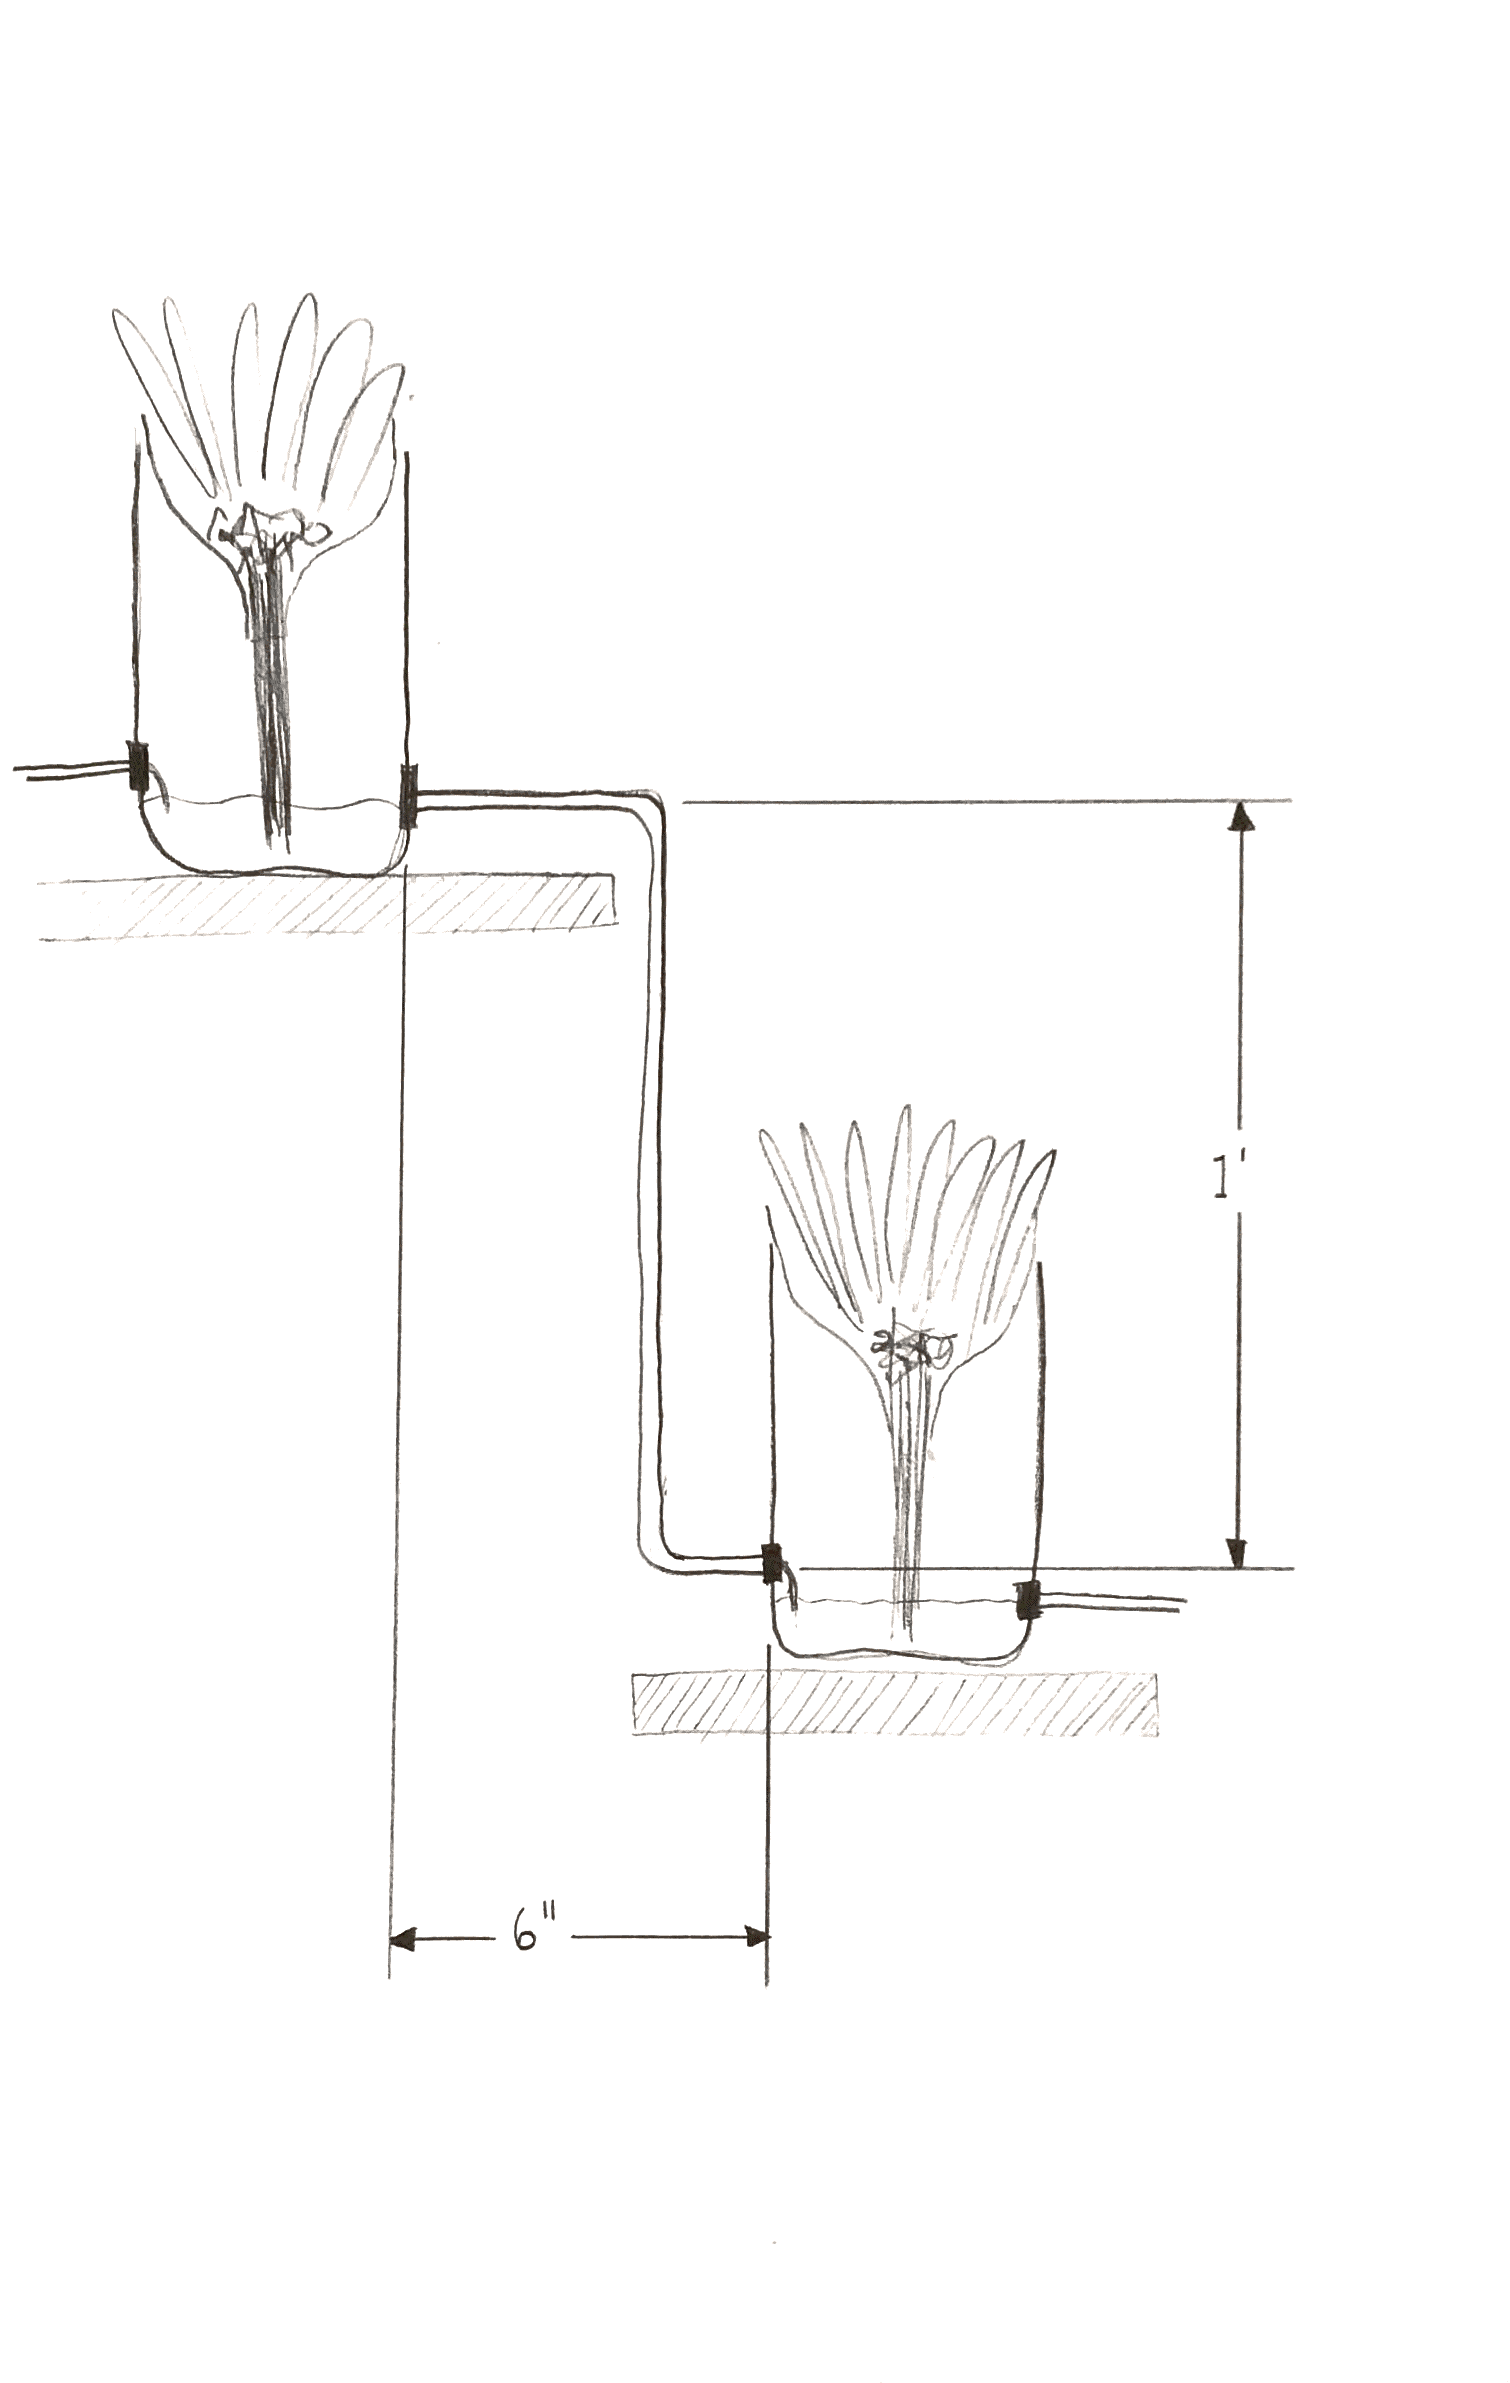
\includegraphics[width=135mm]{resources/tubing-bottle-to-bottle.png}
    \caption{Dimensions of Tubing from Bottle to Bottle to Bottle}
\end{figure}

\section{Subsystem Interfaces}

% Explain the interfaces with the other subsystems: describe each interface and how your design
% addresses each. Reference a figure or a table.
There are two interfaces between the water delivery subsystem and other subsystems:

\begin{enumerate}
    \item The connections to the four reservoirs in the reservoir subsystem.
    \item The connections to and from the twelve hydroponic bottles.
\end{enumerate}

% Reservoir
The interface with the reservoir is twofold. First, the tubing of the water delivery subsystem
attaches to the pump in the reservoir. The tubing also passes through a hole cut in the ceiling of
the reservoir. To ensure that the pump and tubing are compatible with one another,
$\nicefrac{1}{2}''$ tubing is being used. Additionally, the ceiling of the reservoir has a
$\nicefrac{1}{2}''$ hole allowing the tube to pass through. This arrangement allows the stakeholder
to lift lid of the reservoir without having to disconnect any tubing.

% Bottle connection
The interface with the bottle consists of a bulkhead fitting, the $\nicefrac{1}{2}''$ tubing and the
bottle itself. Figure 4 shows this interface. The bulkhead fitting has two parts: the bulkhead
body and the bulkhead locknut. The bulkhead body and the threads are one piece and fit through a
hole in the soda bottle created using the bottle creation tool designed for the hydroponic bottle
subsystem. The bulkhead locknut is threaded and, once tightened, seals the gap between the bulkhead
body and the soda bottle \cite{uspc}. The threads of the bulkhead body also hold the tubing in
place.

\begin{figure}[H]
    \centering
    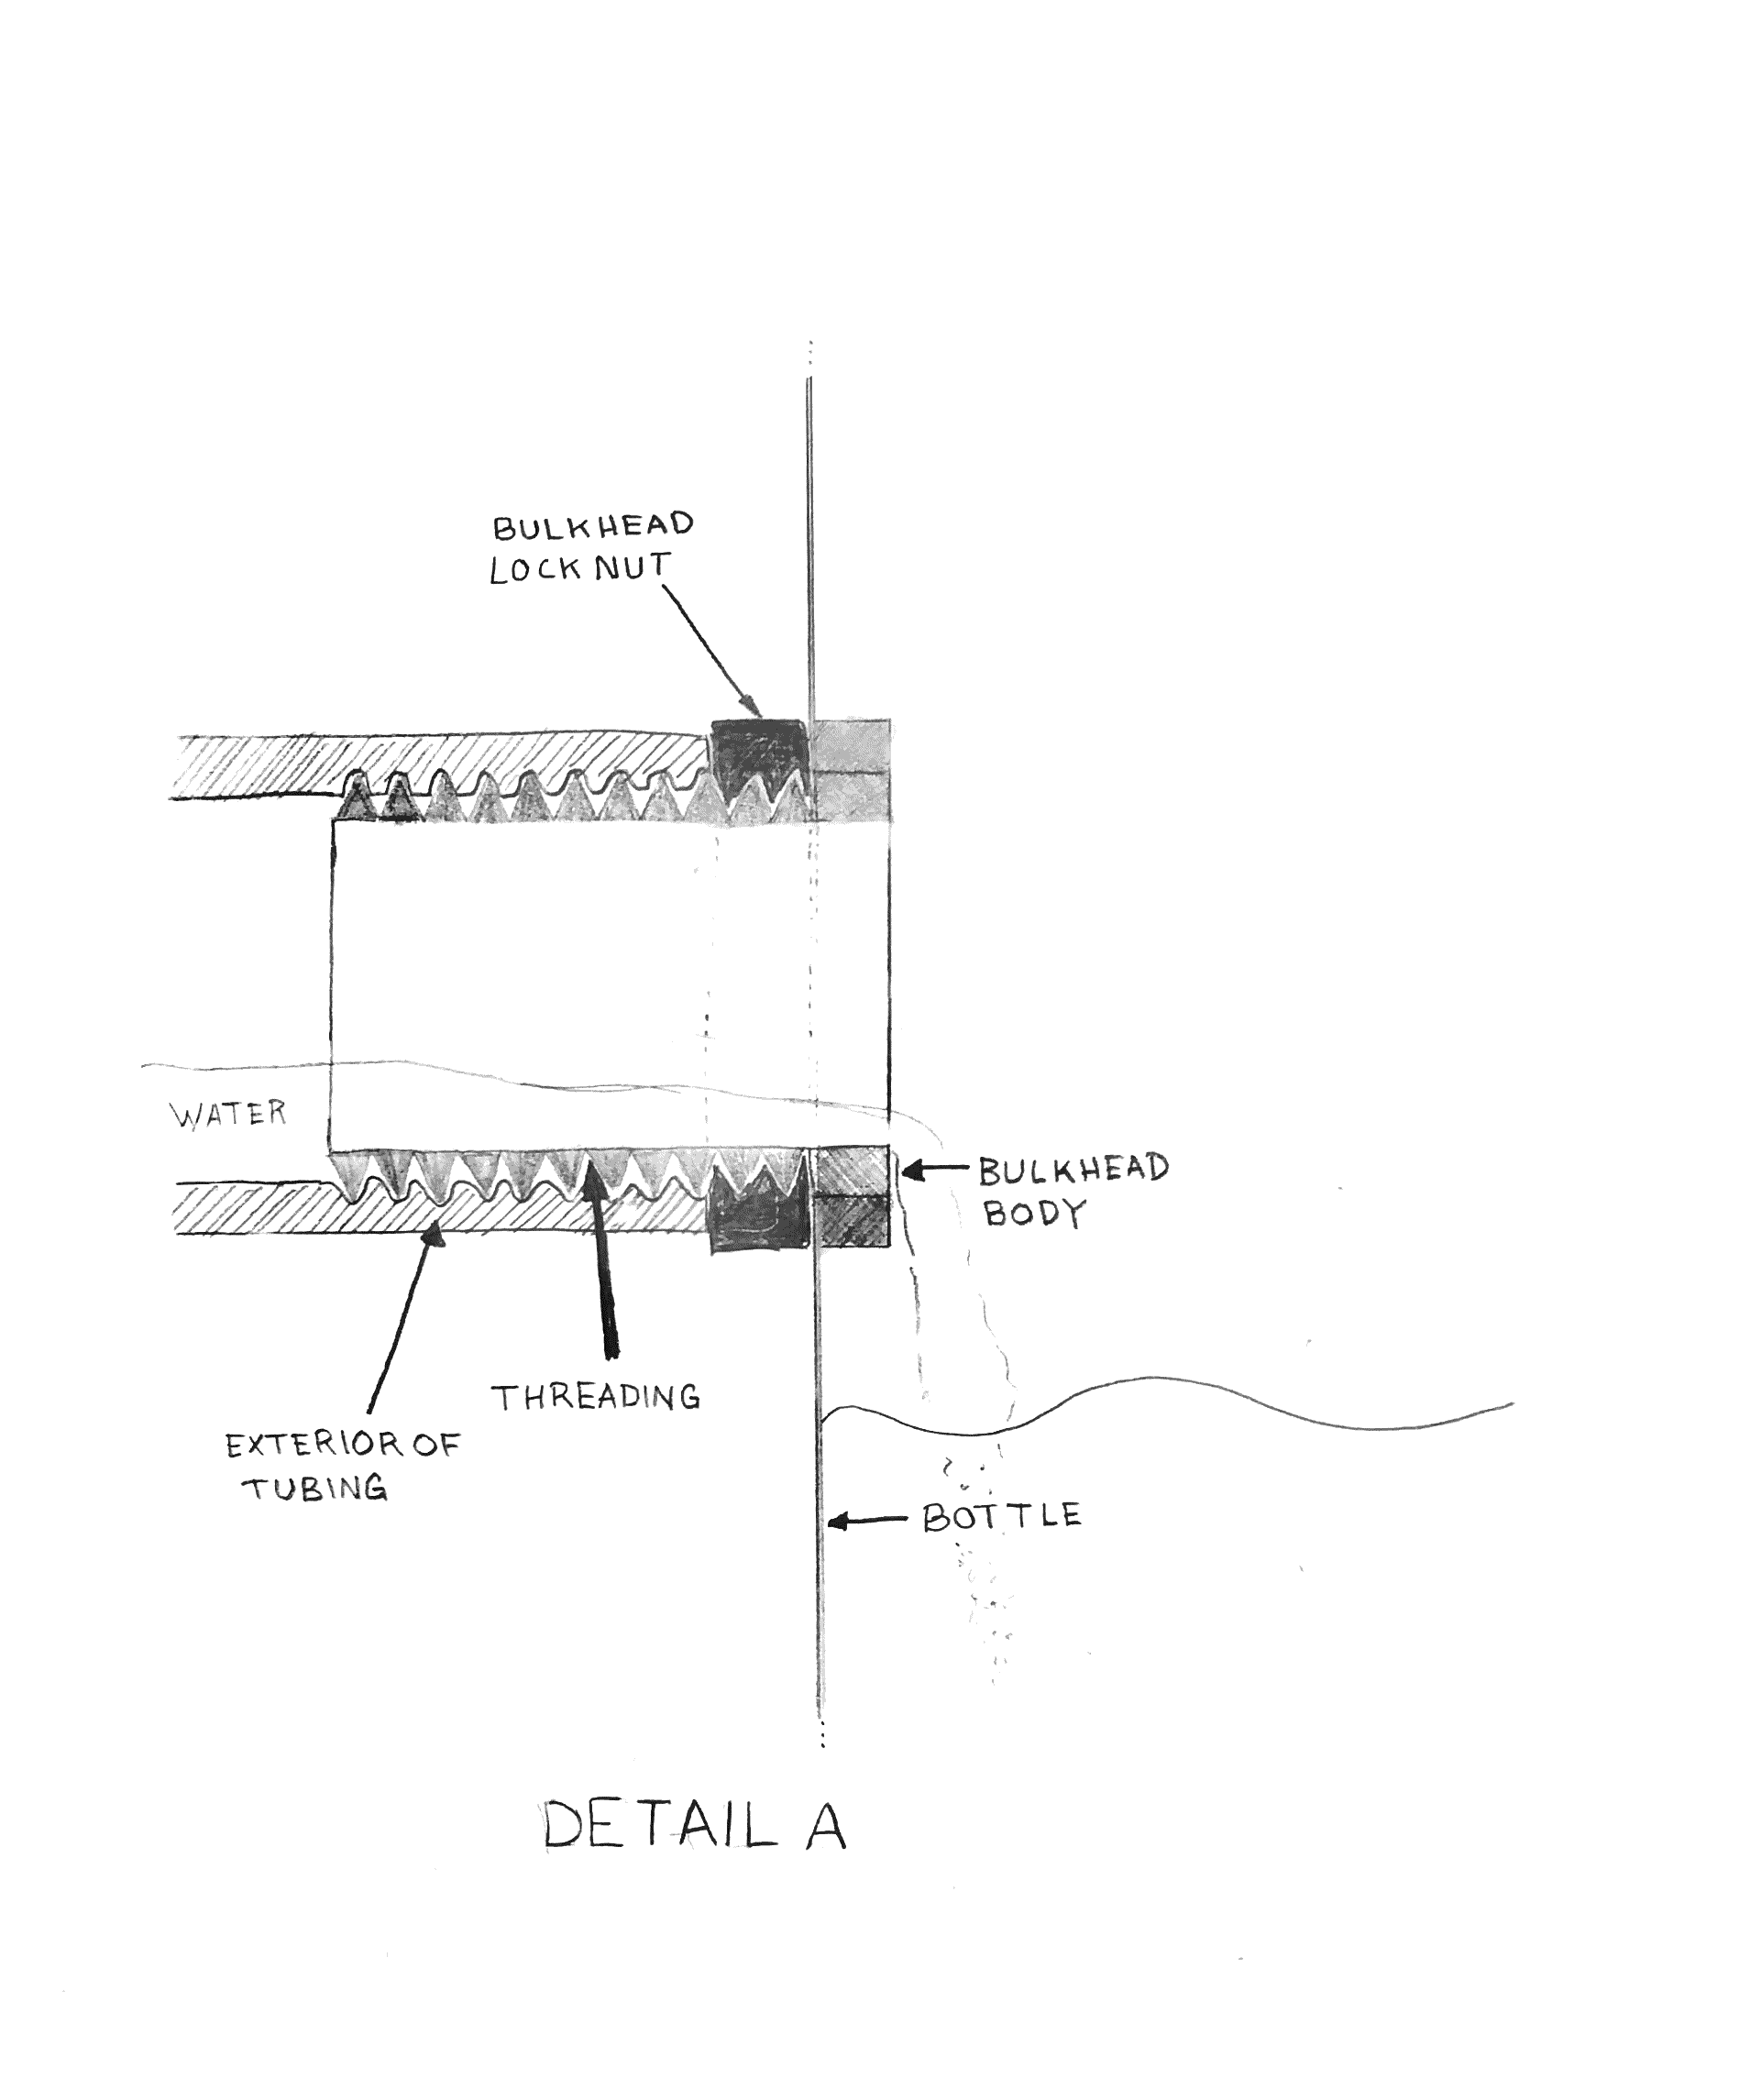
\includegraphics[width=163mm]{resources/detail-a.png}
    \caption{Bulkhead Fitting Connected to Bottle and Tubing}
\end{figure}

\section{Subsystem Analysis}

% Validation that it will work. If tested, what was the design of your experiment/test, and what was
% the result? If not tested, prove through research and analysis that your concept will function as
% planned.

The water delivery subsystem is critical to the overall success of the team's system. Because of
this, extensive testing is required to ensure that the subsystem works. The following is a list of
the tests for the water delivery subsystem that have been identified by the team:

\begin{enumerate}

    \item \textbf{Pump Head:} The pump must have enough head to raise the water from the
        reservoir to the level of the topmost bottle. The team has tested the head of two pumps, the
        \textit{Pondmaster 35 GPH Magnetic Drive Utility Pump} and the
        \textit{EcoPlus\supscr{\textregistered} Eco 66 Bottom Draw 75 GPH}. Unfortunately, both
        pumps had insufficient head. The \textit{Pondmaster} brand pump was only able to raise the
        water about $1'\ 6''$. The team then tested the The \textit{EcoPlus\supscr{\textregistered}}
        brand pump which performed better but was still only able to raise water about $2'\ 6''$.

    \item \textbf{Bottle Connections:} The tubing must fit properly onto the bulkhead fitting
        and the bulkhead fitting must seal the hole in the bottle.

    \item \textbf{Amount of Pump Time Required to Maintain Sufficient Level of Water:} It is
        important that the wicking material (designed as part of the Hydroponic Bottle Subsystem)
        never becomes dry \cite{kaiser-and-erns}. This would occur if the water in the bottom of the
        bottle runs out, thus the water in the hydroponic soda bottles needs to be replenished
        periodically.

\end{enumerate}

\section{Summary}

% Given your research, stakeholder feedback and/or testing, what are your recommendations for
% design iterations and design implementation into the final, full-scale, production solution?

% Testing
After testing the \textit{Pondmaster} brand pump the team assumed that doubling the GPH would double
the head. This assumption was disproved after testing the \textit{EcoPlus\supscr{\textregistered}}
which had over twice the GPH of the \textit{Pondmaster} pump. The team then considered other ways to
increase the head of the pumps that they already had. One idea was to decrease the diameter of the
tubing, increasing pressure in the tube and hopefully pushing the water higher. The team has not
started testing this idea.

If decreasing the tube diameter does not increase the head, the team will find a different pump with
more head. Since the pumps that the team has tested to date are some of the weakest pumps on the
market, finding a pump with sufficient head should not be an issue. Although finding a suitable pump
is critical to the final design, other testing can occur before a pump is found.

The connection from the tubing to the bottles is critical to the overall success of the solution and
thus is the most critical test for the water delivery subsystem. Because of this, these connections
will be tested by November 10, 2016. In the case that the bulkhead fittings do not seal the holes in
the bottle well enough, other options such as trying to utilize the built-in threads on the soda
bottle may be considered.

In the final product, all of the fittings will, in addition to being watertight, need to be easy
to install so that the stakeholder can create the bottle with limited technical knowledge. Because
of this, the team will test for leakage by performing a stress test. This stress test involves
turning the pump on for 12 hours and measuring any leakage through the bulkhead fittings. From
previous testing, the team has found that installing bulkhead fittings is relatively easy and can be
done without much technical knowledge.

In summary, the water delivery subsystem is essential to the functionality of the overall system.
Although the team's research and testing to-date has indicated that this subsystem is viable, the
water delivery subsystem will require extensive testing to ensure that it interfaces correctly with
the other subsystems.

\pagebreak

\begin{thebibliography}{9}
    \bibitem{cdc-food-deserts}
    Centers for Disease Control and Prevention (2012).
    \textit{A Look Inside Food Deserts} [Online].
    Available: \url{http://www.cdc.gov/features/FoodDeserts/index.html}.
    [Accessed Sept. 11, 2016].

    \bibitem{usda-food-deserts}
    United States Department of Agriculture Economic Research Service (19 Oct. 2016).
    \textit{Food Access Research Atlas} [Online].
    Available:
    \url{http://www.ers.usda.gov/data-products/food-access-research-atlas/go-to-the-atlas.aspx}.
    [Accessed: Oct. 28, 2016].

    \bibitem{j-camas}
    J. Camas (04 Sept. 2014).
    \textit{Home Hydroponics} [Online].
    Available:
    \url{http://www.epicurious.com/archive/blogs/editor/2014/09/home-hydroponics-easy-tips-for-growing-fresh-produce-all-year.html}.
    [Accessed: Nov. 2, 2016].

    \bibitem{doe-washington}
    Washington State Department of Ecology.
    \textit{Algae Information} [Online].
    Available: \url{http://www.ecy.wa.gov/programs/wq/plants/algae/lakes/AlgaeInformation.html}.
    [Accessed: Oct. 19, 2016].

    \bibitem{uspc}
    United States Plastic Corp (2008).
    \textit{How does a bulkhead fitting work?} [Online].
    Available: \url{http://www.usplastic.com/knowledgebase/article.aspx?contentkey=437}.
    [Accessed: Nov. 3, 2016].

    \bibitem{kaiser-and-erns}
    Cheryl Kaiser and Matt Erns.
    University of Kentucky College of Agriculture, Food and Environment (2012).
    \textit{Hydroponic Lettuce} [PDF].
    Available: \url{http://www.uky.edu/Ag/NewCrops/introsheets/hydrolettuce.pdf}.
    [Accessed: Nov. 03, 2016]

\end{thebibliography}

\end{document}
